\documentclass[11pt]{article}
% Paper (2026-10-04). Sectionised: sections/*.tex. Portable to elsarticle (ATE),
% Cambridge (DCE) or a workshop style with minor edits. Numbers of record:
% torch pipeline, runs/outer (raw-data metrics, IC-fair baselines).
% Figures: docs/paper/figures/*.pdf, generated by scripts/make_paper_figures.py
% (publish style: 300 dpi + vector PDF, Okabe-Ito palette, 8 pt serif).
\usepackage[margin=2.5cm]{geometry}
\usepackage{amsmath,amssymb}
\usepackage{graphicx}
\usepackage{booktabs}
\usepackage{siunitx}
\usepackage[hidelinks]{hyperref}
\graphicspath{{figures/}}
\sisetup{detect-all}

\title{A Physics-Informed Grey-Box Model of an Oscillating Heat Pipe:\\ Identification, Extrapolation, and Working-Fluid Coupling Ratios}
\author{Jaminur Rahman Khalid}
\date{}

\begin{document}
\maketitle
\begin{abstract}
Choosing a working fluid for oscillating heat pipes (OHPs) usually requires a separate experiment per candidate, and
the underlying two-phase flow resists first-principles modelling. We identify a physics-informed grey-box model of a
helically coiled OHP from transient temperature measurements of one apparatus operated with ethanol, methanol and
deionised water, each in three heating runs (vessel plateaus $\sim$58, $\sim$70, $\sim$\SI{93}{\celsius}; nine
run--fluid series). A lumped two-node energy balance, driven by the measured vessel temperature, is fitted by a
physics-informed neural network (PINN), which learns the physical parameters jointly with the temperature curves
through the ODE residual, and equally by plain ODE shooting. Under leave-one-run-out validation the identified model
predicts the evaporator temperature of an unseen run at \SIrange{0.24}{0.46}{\kelvin} when interpolating and
\SIrange{0.71}{0.85}{\kelvin} when extrapolating (up or down) in heating level. Reference baselines given the same
measured initial state locate what this tests: a trivial constant-gap predictor stays within \SI{3}{\kelvin};
nonlinear black boxes (multilayer perceptron, Gaussian process, degree-2 SINDy) reach \SIrange{0.6}{6}{\kelvin}
on the interpolation fold but fail at \SIrange{24}{87}{\kelvin} on extrapolation, with a recurrent GRU best among them at
\SI{5}{\kelvin}; a one-node ablation of the same ODE matches the two-node fits on the evaporator, so the second node
is justified by the condenser and adiabatic channels, not by evaporator accuracy; and an unconstrained per-fluid
linear state-space with no physical parameterisation matches or beats the physical model in every fold -- the
linear structure, fitted by output-error shooting, is what carries extrapolation, and the physical
parameterisation is retained for parsimony and interpretability. Plain ODE shooting is slightly
better than the PINN in every fold: for this fully observed 9-parameter linear system the structure, not the
optimiser, carries the accuracy. A dimensionless coupling ratio $R^*=a_f/\kappa_f$, identifiable also from plateau
ratios, ranks the fluids in every fit (EOHP $\approx$ 12.6--13.5 $>$ MOHP $\approx$ 7.1--7.3 $>$ WOHP $\approx$
5.8--6.0); its $\sim$48\% drift for ethanol across heating levels is consistent with the ethanol dry-out reported in
the source study, a regime the constant-parameter model cannot represent; a per-run temperature-dependent
$\kappa(T_e)$ is identifiable but does not transfer across heating levels, so the deployed model keeps $\kappa$
constant. The fitted right-hand side exports as
ONNX; scenario sweeps within the validated envelope illustrate model-implied trade-offs between setpoint tracking
and ripple rejection along $R^*$, and are explicitly not fluid recommendations. Limitations: one geometry, one
shared driver per run, slow ramps, \SI{5}{\second} sampling, equal vessel--evaporator coupling assumed, and no
heat-flux or dry-out limits.
\end{abstract}

\section{Introduction}
Oscillating heat pipes (OHPs) achieve high effective conductivity through self-excited two-phase oscillation, but the
same mechanism makes their behaviour difficult to model from first principles: the flow regime, the distribution of
liquid slugs and vapour plugs, and the evaporation--condensation dynamics are only partially observable through wall
temperatures. Working-fluid comparison is therefore usually experimental: one apparatus per fluid, per fill ratio, per
geometry. Data-driven surrogates trained on such measurements interpolate well but are known to fail when asked to
extrapolate to unseen operating conditions -- precisely the question a designer asks (``what if we run hotter?'').

Grey-box identification offers a middle road: impose the physically mandatory structure (energy conservation on a
small number of lumped nodes) and learn the few effective parameters from data. Physics-informed neural networks
(PINNs) provide a convenient machinery for this, embedding the ODE residual in the loss through automatic
differentiation and optimising physical parameters jointly with a trial solution. What PINNs add over classical
shooting-based parameter fitting for such small, well-posed ODEs is, however, an open and often glossed-over question.

This paper contributes a deliberately honest case study on a public dataset of a helically coiled OHP (HCOHP)
\cite{dataset,dib} operated with three working fluids:
\begin{enumerate}
  \item a two-node grey-box model, vessel-temperature-driven, identified by PINN and by ODE shooting, validated
        leave-one-run-out with extrapolation both up and down in heating level, against IC-fair baselines:
        trivial, linear, and nonlinear black boxes (MLP, GP, SINDy, autoregressive GRU);
  \item evidence that a correctly structured linear model, not the PINN optimiser or the physical
        parameterisation, carries the accuracy: shooting, one-node, and even an unconstrained per-fluid linear
        state-space extrapolate at \SIrange{0.3}{0.9}{\kelvin} while nonlinear black boxes degrade
        (GRU \SI{5}{\kelvin}, others \SIrange{24}{87}{\kelvin}; trivial gap baseline \SI{3}{\kelvin});
  \item a dimensionless coupling ratio $R^*=a_f/\kappa_f$ that is invariant to the sampling interval,
        seed- and method-stable, ranks the fluids identically in every fit, and is recoverable from plateau
        ratios alone -- with the ethanol drift consistent with the dry-out reported in the source data;
  \item negative results reported as such: a temperature-dependent pipe conductance $\kappa(T_e)$ is
        identifiable within each run (an initial ``not identifiable'' verdict was an optimiser artefact,
        corrected) but is a heating-level effect that does not transfer across runs, so the deployed model
        keeps $\kappa$ constant; per-fluid condenser loss rates do not pay for their parameters;
  \item a consistency check on an untrained channel: adiabatic-section temperatures are reproduced as a static
        mixture of the two identified nodes to \SI{<0.5}{\kelvin} on held-out EOHP/WOHP runs (MOHP is harder);
  \item an exported ONNX simulator used for model-implied scenario illustrations (tracking vs.\ ripple rejection
        along $R^*$) with seed-ensemble bands -- explicitly not fluid recommendations, since the model carries no
        heat-flux or dry-out limits.
\end{enumerate}

\section{Related work}
\textbf{Oscillating heat pipes.} OHPs (pulsating heat pipes) are reviewed comprehensively in \cite{ma2015}; their
effective behaviour emerges from self-excited two-phase oscillation that resists first-principles modelling, which
is why thermal-performance studies largely remain experimental and apparatus-specific. Our data source, the HCOHP
study of Yeboah and Darkwa \cite{ijts,dataset,dib}, is unusual in publishing raw thermocouple records for three
working fluids under three heating levels, and in reporting fluid-dependent dry-out onset (ethanol first) --
the phenomenon our constant-parameter model structurally cannot represent, and which any fluid-selection use of
these models must confront \cite{li2019}. The common engineering metric is a steady thermal resistance
$R_{th} = (T_e - T_c)/Q$ \cite{li2019,ijts}; our $R^*$ is deliberately dimensionless (a ratio of identified rates,
recoverable from plateau ratios) because absolute fluxes are not identifiable from these records.

\textbf{Grey-box identification.} Imposing physically motivated structure on a low-dimensional state-space and
fitting its parameters from data is classical system identification \cite{ljung}. The methodological points we
lean on are old and robust: parameter sloppiness (stiff ratios, sloppy rates) is generic in multi-parameter
physical models \cite{gutenkunst}, which is why we report the ratio $R^*=a_f/\kappa_f$ rather than the rates; and
structure selection must be validated out-of-sample, which is what the LORO protocol with two extrapolation
directions provides.

\textbf{PINNs for inverse problems.} PINNs embed governing equations in the loss of a neural trial solution
\cite{raissi} and have become a standard tool for forward and inverse problems \cite{karniadakis}. Known
pathologies (gradient flow, optimisation sensitivity) are documented \cite{wang2021}; for small, fully observed
lumped systems the classical alternative -- least-squares shooting over the same equations -- is trivially
available, and controlled comparisons of the two on identical structure are rarer than method papers. Our result
(shooting $\ge$ PINN in every fold, one-node $\approx$ two-node on the target channel) is a data point for that
literature, in the spirit of baseline-honest evaluations.

\textbf{Data-driven dynamics.} SINDy \cite{brunton} and GPs \cite{gp} represent the equation-discovery and
nonparametric-regression routes; our GRU baseline the sequence-learning route. Their uniform failure on the
extrapolation fold (while a trivial constant-gap predictor stays within \SI{3}{\kelvin}) echoes the general point
that interpolation skill does not transfer across operating regimes. The conformal prediction literature
\cite{vovk} offers distribution-free predictive bands; our seed ensembles quantify only parameter uncertainty,
and we mark conformal augmentation as future work rather than claim calibrated bands.

\section{Data}

\begin{figure}[t]\centering
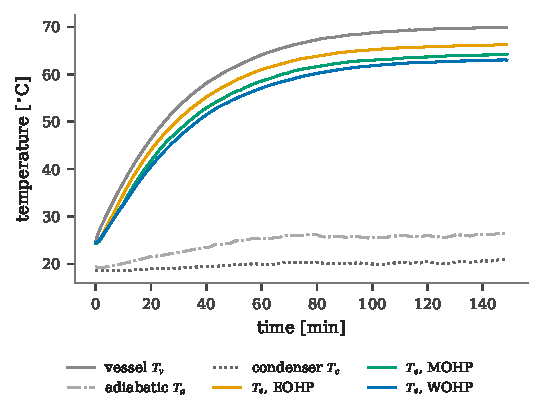
\includegraphics[width=0.5\textwidth]{fig1_data.pdf}
\caption{Raw thermocouple channel means for Run 2 (all three fluids); the vessel/adiabatic/condenser channels are
shared across fluids within a run (common bath), so they are shown once.}
\label{fig:data}
\end{figure}

We use the public HCOHP dataset of Yeboah and Darkwa \cite{dataset,dib}: a copper helical coil (2\,mm ID tube,
\SI{8}{\centi\metre} coil diameter, 10 turns; evaporator/adiabatic/condenser sections 0.19/0.20/0.19\,m) on a heated
vessel (L\,=\,0.30\,m), instrumented with K-type thermocouples logged at \SI{5}{\second}. Three working fluids --
ethanol (EOHP), methanol (MOHP), deionised water (WOHP) -- were each tested in three heating runs reaching vessel
plateaus of approximately 58, 70 and \SI{93}{\celsius} (Fig.~\ref{fig:data}). Per (run, fluid) we form channel
means: vessel $T_v$ (outer wall, the driver), evaporator $T_e$ (3 TCs), condenser $T_c$ (3 TCs), adiabatic $T_a$
(2 TCs). Models are fitted on Savitzky--Golay-smoothed, 25\,s-subsampled series; all reported errors compare
predictions interpolated onto the raw unsmoothed records.

\section{Model and identification}
\subsection{Two-node grey-box structure}
With the measured vessel temperature as exogenous driver, per fluid $f$:
\begin{align}
\dot T_e &= a_f\,(T_v - T_e) - \kappa_f\,(T_e - T_c), &
\dot T_c &= r\,\kappa_f\,(T_e - T_c) - d\,(T_c - T_{\mathrm{cool}}),
\label{eq:ode}
\end{align}
where $a_f$ is the vessel--evaporator coupling over evaporator heat capacity, $\kappa_f$ the pipe conductance over
the same capacity, $r=C_e/C_c$, $d$ a condenser loss rate, and $T_{\mathrm{cool}}$ the sink temperature; $r$, $d$,
$T_{\mathrm{cool}}$ are shared across fluids. The dimensionless quantity
\begin{equation}
R^* \;=\; \frac{R_{\mathrm{pipe}}}{R_{\mathrm{in}}} \;=\; \frac{a_f}{\kappa_f}
\label{eq:rstar}
\end{equation}
requires no knowledge of the evaporator heat capacity and is the natural per-fluid output of the identification.
We assume the vessel--evaporator coupling geometry is common to the three pipes ($a_f$ differences are fluid-side);
within-run vessel inner/outer thermocouples are identical across fluid sheets, consistent with a shared bath
measurement, and the plateau $T_v{-}T_e$ ordering matches the fitted $a$ ordering.

\subsection{PINN}
A small trial network $U_\theta(t, \text{series})\to(T_e,T_c)$ (3$\times$64 tanh MLP) is trained on the smoothed
thermocouple data plus the ODE residual of Eq.~\eqref{eq:ode}, evaluated on $U$ by autodiff in time; the physical
parameters $(\log a_f, \log\kappa_f, \log r, \log d, T_{\mathrm{cool}})$ are optimised jointly (Adam, cosine decay,
6000 steps, float32). A state-dependent variant learns $\log\kappa_f \mathrel{+}= g_f(T_e, T_e{-}T_c)$ with a small
MLP $g$. Ten seeds per fold quantify the fit's parameter dispersion.

\subsection{ODE shooting}
The same Eq.~\eqref{eq:ode} with constant $\kappa_f$ is fitted by least-squares shooting (scipy
\texttt{least\_squares} over log-parameters, LSODA rollouts). This is the classical route; comparing it to the PINN
isolates what the neural machinery contributes.

\subsection{Black-box baselines (IC-fair)}
All baselines receive the same information the physics fits use, including the measured initial state:
(MLP, GP) map $(t, T_v, \dot T_v, \text{fluid one-hot}, T_e(0), T_c(0)) \to (T_e, T_c)$ pointwise;
SINDy (STLSQ, degree-2 polynomial library in $(T_e,T_c)$ with $T_v$ and fluid one-hot as control, states std-scaled,
time in hours) is integrated by clipped RK4 rollout from the measured initial state; the GRU baseline is an
autoregressive dynamical model (GRU cell, hidden 64) consuming $(t, T_v, \dot T_v, \text{fluid}, T_e^{\mathrm{prev}},
T_c^{\mathrm{prev}})$, trained teacher-forced one-step-ahead (25\,s steps) and rolled out from the measured initial
state, driven by the measured $T_v(t)$. Three GRU seeds; GP with wide kernel bounds ($10^{-3}$--$10^{4}$,
5 restarts) is reported as GP.

Four further references probe what the comparison actually tests:
\textbf{Trivial} $T_e = T_v - c_f$ (per-fluid mean gap); \textbf{Ridge-linear}, a linear state-space
$\dot{(T_e,T_c)} = W\,[T_e, T_c, T_v, \text{fluid}, 1]$ fitted by ridge regression on finite-difference
derivatives and rolled out by RK4 (the linear data-driven counterpart); a \textbf{one-node} ablation
$\dot T_e = a_f(T_v - T_e) - d\,(T_e - T_{\mathrm{cool}})$ fitted by the same shooting procedure (five parameters,
no condenser node; predicts $T_e$ only); and \textbf{Linear-SS}, an unconstrained per-fluid linear state-space
$\dot X = A X + g\,T_v + c$ with all eight entries free per fluid (no cross-fluid or physical sharing),
fitted by the same output-error shooting -- a free linear form of the same order as the physical model.

\subsection{Validation protocol}
Leave-one-run-out (LORO): fit on six (run, fluid) series of two runs, predict all three fluids of the held-out run by
rolling the identified ODE (or GRU) from its measured initial state, driven by its measured $T_v(t)$. Because the
three fluids within a run share the same vessel drive, each fold has effectively one independent driver with three
repeated measures. Only holding out Run 2 is interpolation; Run 1 is downward extrapolation (training on
$\sim$70 and $\sim$\SI{93}{\celsius}, testing at $\sim$\SI{58}{\celsius}) and Run 3 upward extrapolation
(training $\le$\SI{70}{\celsius}, testing $\sim$\SI{93}{\celsius}). Structure-selection choices made during the
analysis (constant $\kappa$, shared $d$, driver variant, $T_c$ weighting) were made with all folds in view and are
therefore not blind; the $\kappa(T_e)$ assessment rests on fixed-$\beta$ grid profiles with the remaining
parameters refit at every grid point (within-run identifiability) and on two-run LORO transfer fits.
A final fit on all runs provides the deployed model.

\section{Results}

\begin{figure}[t]\centering
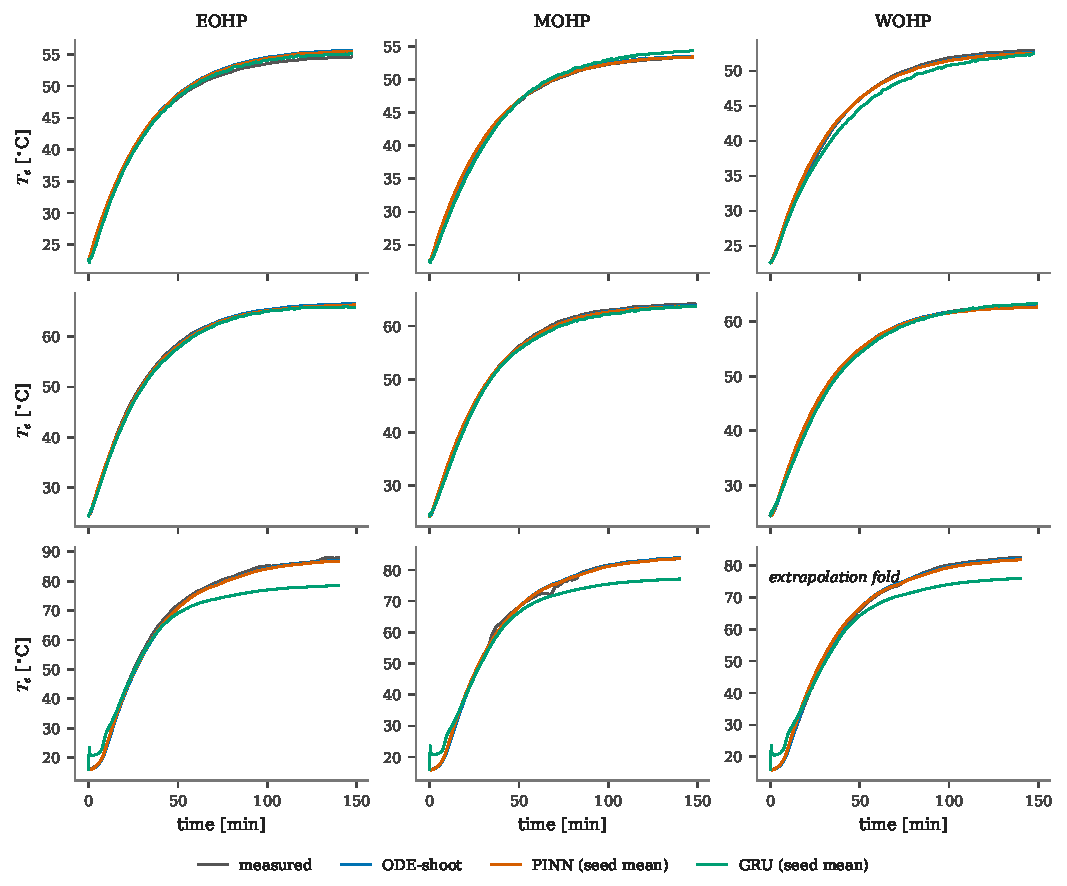
\includegraphics[width=\textwidth]{fig2_loro.pdf}
\caption{LORO held-out evaporator predictions (all folds and fluids): measured (black), ODE shooting (blue),
PINN-const seed-mean (vermillion), GRU seed-mean (green). Run 3 is the extrapolation fold; black boxes degrade
there, structured fits do not.}
\label{fig:loro}
\end{figure}

\begin{figure}[t]\centering
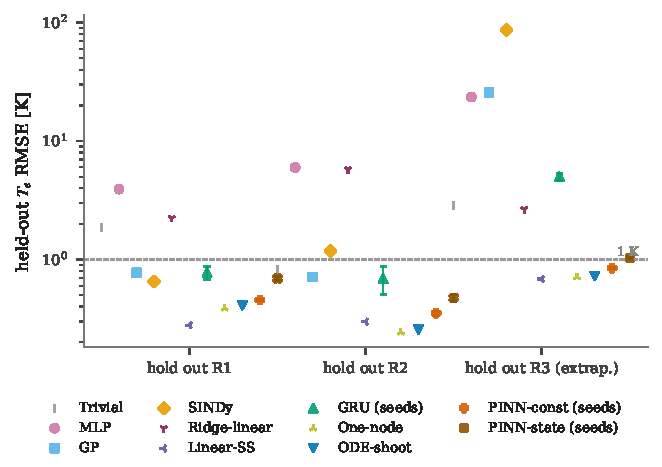
\includegraphics[width=0.7\textwidth]{fig3_rmse.pdf}
\caption{Held-out $T_e$ RMSE by method and fold (mean over fluids; seed sd where applicable; log scale).}
\label{fig:rmse}
\end{figure}

\subsection{Prediction accuracy}
Table~\ref{tab:loro} and Figs.~\ref{fig:loro}--\ref{fig:rmse} give the headline result, and the added references
sharpen what it means. The trivial gap baseline $T_e = T_v - c_f$ is within \SI{3}{\kelvin} everywhere -- the
signal rises some \SI{60}{\kelvin}, so all sub-3\,K numbers should be read against that anchor -- and it beats every
nonlinear black box on the upward-extrapolation fold. What enables extrapolation is \emph{structure}, not physics
specifically: every linear two-state form fitted by output-error shooting extrapolates -- the physical ODE at
0.41/0.26/\SI{0.73}{\kelvin}, the one-node ablation at 0.39/0.24/\SI{0.71}{\kelvin}, and an unconstrained
per-fluid linear state-space with no physical parameterisation at all at 0.28/0.30/\SI{0.68}{\kelvin} -- while
free-form learners (MLP, GP, degree-2 SINDy) fail at \SIrange{23}{87}{\kelvin}. The ridge-fitted linear
state-space sits between (\SIrange{2.7}{5.8}{\kelvin}) because its rates come from noisy finite differences
(errors in variables), not from shooting. The physical parameterisation is therefore unnecessary for
\emph{accuracy}: the free linear form matches or beats it in every fold; it is retained for parsimony (9 shared
parameters against $3{\times}8$ free ones, fitted per fluid without cross-fluid borrowing) and for the
interpretable $R^*$ it exposes. The GRU, exploiting temporal structure, is the best black
box on extrapolation (\SI{5}{\kelvin}) but still $\sim$6$\times$ worse than the structured fits. The ODE shot is
slightly better than the PINN in every fold (0.41/0.26/0.73 vs.\ 0.45/0.35/0.85); for this fully-observed
9-parameter system the PINN machinery adds nothing measurable over classical shooting -- the honest conclusion,
not a surprise. Seed dispersion of the PINN is $\le$\SI{0.03}{\kelvin} across ten seeds per fold.

\begin{table}[t]\centering\small
\caption{Held-out evaporator $T_e$ RMSE (mean over fluids, K) against raw data; mean~$\pm$~sd over seeds.
Run 2 is interpolation; Runs 1 and 3 are downward/upward extrapolation in heating level.}
\label{tab:loro}
\begin{tabular}{lccc}
\toprule
 & Run 1 (down extrap.) & Run 2 (interp.) & Run 3 (up extrap.) \\
\midrule
Trivial ($T_v{-}c_f$) & 1.87 & 0.82 & 2.84 \\
MLP            & 3.93 & 5.98 & 23.54 \\
GP (narrow / wide) & 0.77 / 0.58 & 0.71 / 0.74 & 25.80 / 25.81 \\
SINDy (deg 2)  & 0.65 & 1.19 & 86.49 \\
Ridge-linear   & 2.24 & 5.78 & 2.66 \\
Linear-SS ($3{\times}8$ params) & 0.28 & 0.30 & $\mathbf{0.68}$ \\
GRU (3 seeds)  & $0.77\pm0.09$ & $0.69\pm0.18$ & $\mathbf{4.99\pm0.34}$ \\
One-node (5 params) & 0.39 & 0.24 & 0.71 \\
ODE-shoot (9 params) & 0.41 & 0.26 & 0.73 \\
PINN-const (10 seeds) & $0.45\pm0.01$ & $0.35\pm0.01$ & $0.85\pm0.01$ \\
PINN-state (10 seeds) & $0.69\pm0.02$ & $0.47\pm0.04$ & $1.03\pm0.03$ \\
\bottomrule
\end{tabular}
\end{table}

Condenser $T_c$ RMSE is \SIrange{0.2}{1.5}{\kelvin} for all physics fits ($T_c$ moves only \SIrange{2}{5}{\kelvin}).

\subsection{Structure ablation: is the second node needed?}
The one-node model (5 parameters, no condenser node) matches the two-node fits on $T_e$ everywhere
(0.39/0.24/0.71\,K vs.\ 0.41/0.26/0.73 for shooting). For evaporator prediction alone, the second node, $r$, $d$
and $T_{\mathrm{cool}}$ earn nothing -- the two-node structure is retained because it additionally predicts the
condenser channel and is validated by the adiabatic consistency check below, and because its parameters carry
the physical interpretation; but no accuracy claim rests on the extra node.

\begin{figure}[t]\centering
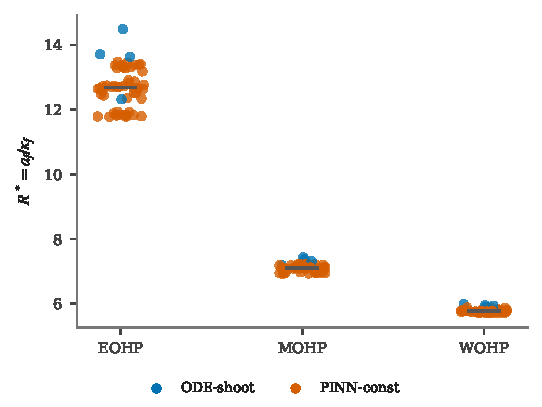
\includegraphics[width=0.6\textwidth]{fig4_rstar.pdf}
\caption{Dimensionless coupling ratio $R^*=a_f/\kappa_f$ from every fit (all LORO folds and seeds).}
\label{fig:rstar}
\end{figure}

\begin{figure}[t]\centering
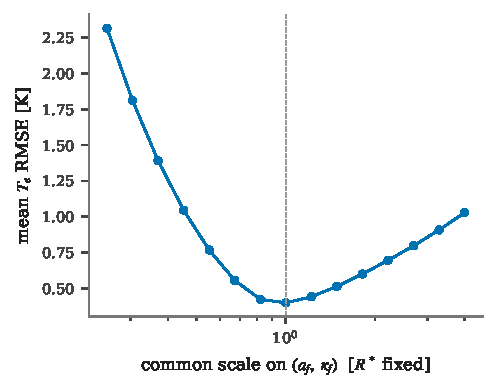
\includegraphics[width=0.5\textwidth]{fig5_ident.pdf}
\caption{Identifiability: rescaling $(a_f,\kappa_f)$ jointly (fixed $R^*$) barely moves the held-out RMSE -- the
rates are sloppy, their ratio is not. The absolute rates still set scenario timescales; that band is propagated
in the scenario metrics below.}
\label{fig:ident}
\end{figure}

\subsection{Identified parameters and \texorpdfstring{$R^*$}{R*}}
$R^*$ (Table~\ref{tab:rstar}, Fig.~\ref{fig:rstar}) ranks EOHP $>$ MOHP $>$ WOHP in every fit and every fold. It is
a ratio of fitted rates and we do not attribute it to a specific resistance: the decomposition between
vessel--evaporator contact resistance and pipe resistance is not identifiable here, and the source study reports
fluid-dependent contact resistance. Quantitatively, in the final shooting fit $\ln R^*_E/R^*_W = 0.83$ splits as
$\ln(a_E/a_W) = +0.54$ minus $\ln(\kappa_E/\kappa_W) = -0.29$: about two-thirds of the gap sits in the inlet
coupling $a_f$ and one-third in the pipe conductance $\kappa_f$ (PINN: 60/40;
runs/outer/rstar\_decomposition.log). These shares are per-fluid ratios of fitted rates, hence invariant to the
joint-rescaling sloppiness of Fig.~\ref{fig:ident}, but they remain a decomposition of fitted rates, not
measurements of separate physical resistances.
In steady state $R^* = (T_e{-}T_c)/(T_v{-}T_e)$, and plateau ratios computed directly from the data give
9.9/12.4/14.6 (EOHP), 7.1/7.6/7.2 (MOHP), 6.4/6.1/6.1 (WOHP) for Runs 1--3 -- the dynamics-based fit reproduces
the plateau ratios and smooths their run-to-run drift. That drift is informative: EOHP's ratio rises $\sim$48\%
with heating level while methanol and water stay flat, consistent with the early, sharp ethanol dry-out reported
in the source study (onset 70/83/98\,W for ethanol vs.\ 105/135/160\,W gradual onset for methanol and water); the
constant-$\kappa$ model absorbs this as a cross-run power-level effect ($\pm$20\% on $\kappa$) and cannot represent
dry-out onset. $R^*$ is invariant to the sampling interval (DT$_S$\,=\,1 vs 5 reruns give identical rankings and
near-identical values), and robust to the choice of vessel thermocouple driver (outer vs.\ mean-of-four changes
absolute values by up to $\sim$12\% but never the ranking or the accuracy). The absolute rate parameters
$(a_f,\kappa_f)$ are constrained only to within a factor $\sim$2 at the sub-kelvin level -- rescaling both jointly
leaves RMSE at 0.40/0.65\,K for 1$\times$/2$\times$ (Fig.~\ref{fig:ident}) -- while their ratio is far stiffer
across methods, seeds and folds; this is why $R^*$, not the rates, is the reportable quantity.

\begin{table}[t]\centering\small
\caption{Dimensionless coupling ratio $R^*=a_f/\kappa_f$ (mean $\pm$ sd over all LORO + final fits).
The ODE-shoot jackknife-over-series row gives 68\% intervals: $R^*$ = 13.6 $\times/\div$ 1.12 (EOHP),
7.3 $\times/\div$ 1.03 (MOHP), 5.9 $\times/\div$ 1.01 (WOHP).}
\label{tab:rstar}
\begin{tabular}{lccc}
\toprule
 & EOHP & MOHP & WOHP \\
\midrule
ODE-shoot    & $13.54\pm0.90$ & $7.33\pm0.11$ & $5.95\pm0.03$ \\
PINN-const   & $12.63\pm0.56$ & $7.09\pm0.09$ & $5.76\pm0.03$ \\
\bottomrule
\end{tabular}
\end{table}

Jackknife-over-series refits of the shooting model (9 leave-one-series-out fits; runs/outer/jackknife.csv)
give series-level uncertainty on the ordering: $\log R^*_E - \log R^*_M = 0.62 \pm 0.11$ and
$\log R^*_M - \log R^*_W = 0.21 \pm 0.03$ (5.4 and 8.2 $\sigma$; 95\% $t$-intervals with 8 degrees of
freedom $[0.36, 0.89]$ and $[0.15, 0.27]$, both excluding zero), i.e.\ the fluid ordering survives
resampling at every level we can test, though with one shared driver per run these are series-level,
not experiment-level, intervals.

\subsection{Negative and corrected results}
\textbf{$\kappa(T_e)$: identifiable within runs, not transferable across them.} An earlier draft of this analysis
reported a per-fluid Arrhenius-type $\kappa_f(T_e)=k_{0f}e^{\beta_f(T_e-50)}$ as ``not identifiable''; that verdict
was an optimiser artefact (the within-run fits initialised $\beta$ at exactly zero with a relative finite-difference
step, which stalls there). Fixed-$\beta$ grid profiles with the remaining five parameters refit at every point
(runs/outer/kappa\_te\_profile.log) show $\beta$ is clearly identifiable \emph{within} a run: ethanol improves
within-run RMSE by 67--71\% at $\hat\beta\approx+0.03$ (19\% in Run 3), water by 45--48\% at
$\hat\beta\le-0.02$ (grid edge), methanol not at all ($\hat\beta\approx0$) -- a sign pattern consistent with the
cross-run $\kappa$ drift. What fails is \emph{transfer}: fitted on two runs with all parameters shared and applied
to the held-out run, the training $\hat\beta$ collapses toward zero and leaves held-out RMSE unchanged or worse in
eight of nine folds (WOHP Run 1: \SI{0.15}{\kelvin} at $\beta=0$ vs.\ \SI{0.52}{\kelvin} at the training
$\hat\beta=-0.005$; one fold improves, EOHP Run 3: 0.77$\to$\SI{0.50}{\kelvin}), and the joint PINN-kTe fit
likewise degrades the extrapolation fold (0.85$\to$\SI{1.19}{\kelvin}). The temperature dependence is thus
run-specific -- a heating-level effect, not a transferable fluid property -- so the deployed model keeps $\kappa$
constant; extrapolating a $\beta$ identified at one power level to another remains open.
\textbf{Per-fluid $d$ unnecessary.} Freeing the condenser loss rate per fluid yields $\le$0.02\,K gains on
interpolated folds and none on extrapolation; learned $d$ ratios span only $\sim$1.2.

\subsection{Adiabatic-channel consistency check}

\begin{figure}[t]\centering
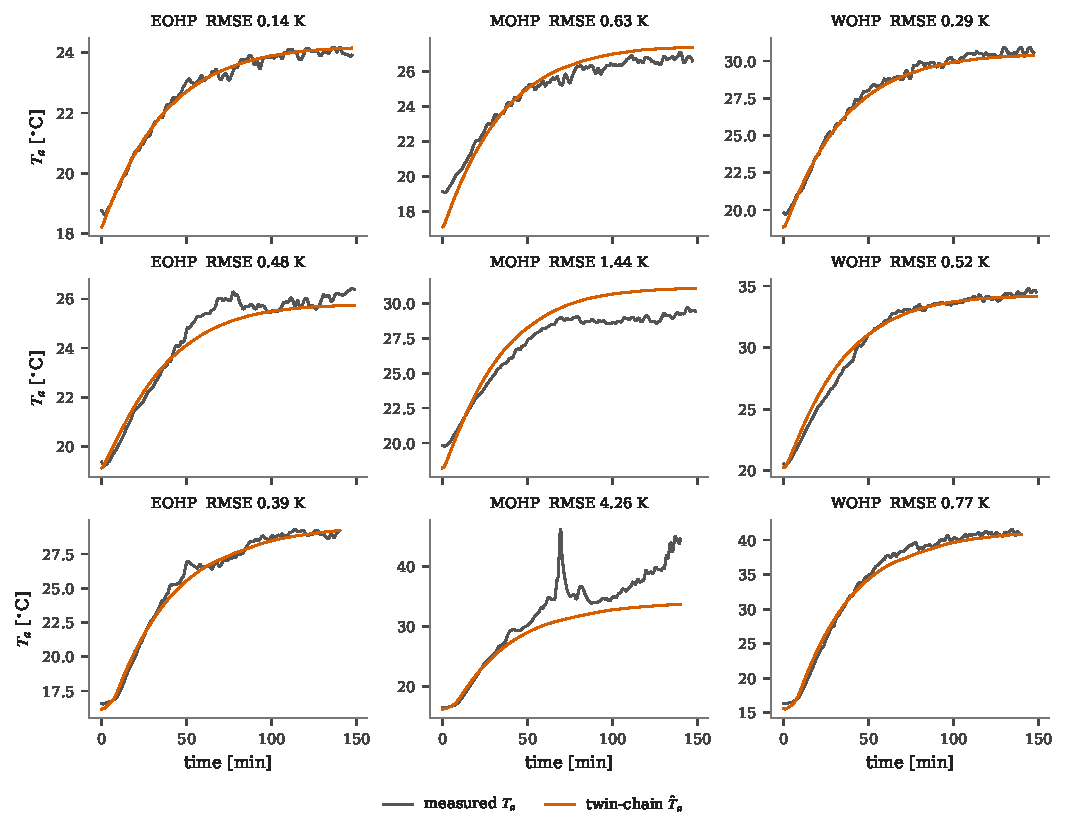
\includegraphics[width=\textwidth]{fig8_adiabatic.pdf}
\caption{Held-out adiabatic channel (never fitted): measured $T_a$ vs.\ the chained prediction
$T_a = w_1 T_e^{\mathrm{pred}} + w_2 T_c^{\mathrm{pred}}$, with $(w_1, w_2)$ fitted on the training runs only.
EOHP and WOHP agree at sub-\SI{0.5}{\kelvin} RMSE; MOHP Run 3 is the identified hard case.}
\label{fig:adiabatic}
\end{figure}

The adiabatic thermocouples were never used in fitting. A static mixture of the two node temperatures,
$T_a \approx w_1 T_e + w_2 T_c$ (no intercept), reproduces them in-sample at \SIrange{0.1}{0.4}{\kelvin} (vs.\
\SIrange{19}{47}{\kelvin} for $T_v$ alone), with $w_1{+}w_2 \approx 0.96$--0.99 and $w_1$ fluid-ordered
(E 0.14 $<$ M 0.24 $<$ W 0.34: the adiabatic wall sits nearer the condenser for water). Under LORO, held-out $T_a$
is predicted at \SIrange{0.27}{0.45}{\kelvin} for EOHP/WOHP and \SIrange{0.6}{3.5}{\kelvin} for MOHP (Run 3 is the hard
case); chaining model-predicted $T_e, T_c$ (Fig.~\ref{fig:adiabatic}) stays at \SIrange{0.14}{0.76}{\kelvin} for E/W
and \SI{4.25}{\kelvin} for MOHP Run 3. We present this as a consistency check, not a structural test: two free
weights can interpolate any profile lying between the two nodes, and the chained version scoring slightly better
than the measured-input version (0.14 vs.\ 0.27\,K for EOHP Run 1) shows the metric is insensitive at this level.
A one-parameter variant ($w_2 = 1 - w_1$, $w_1$ = 0.12/0.20/0.32 for E/M/W) performs the same or better on
EOHP/WOHP (\SIrange{0.17}{0.58}{\kelvin} held-out), confirming the check constrains little beyond ``$T_a$ lies between
the nodes''. It does establish that the fitted two-node states are mutually consistent with an untrained
measurement.

\subsection{Exported model and a model-implied scenario illustration}

\begin{figure}[t]\centering
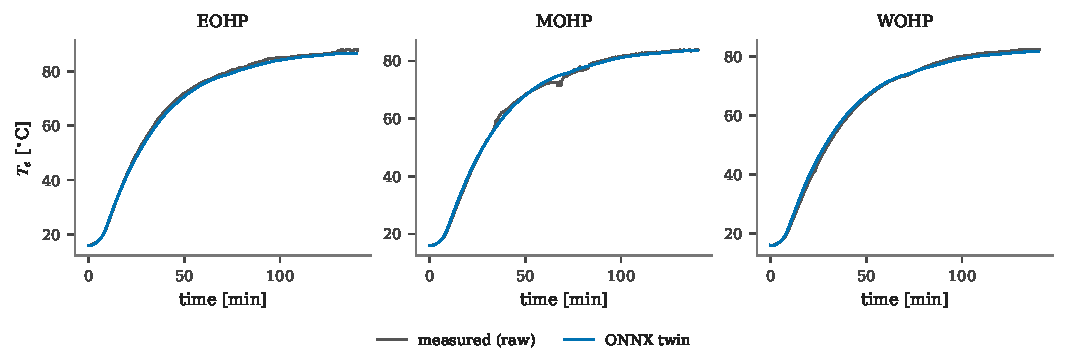
\includegraphics[width=\textwidth]{fig6_replay.pdf}
\caption{Streaming ONNX replay of held-out Run 3 (fold-3 model, never trained on Run 3).}
\label{fig:replay}
\end{figure}

\begin{figure}[t]\centering
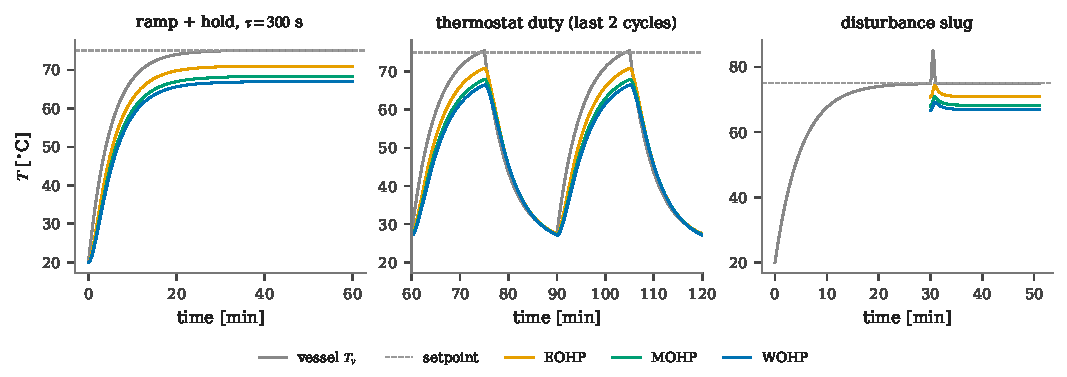
\includegraphics[width=\textwidth]{fig7_case.pdf}
\caption{Model-implied scenarios at a \SI{75}{\celsius} setpoint (ONNX rollouts, final fit). (a) Ramp-and-hold
($\tau=\SI{300}{\second}$): EOHP tracks the vessel tightly (lowest lag, fastest settle); WOHP lags most.
(b) Thermostat on/off duty (last two cycles): WOHP shows the smallest evaporator ripple. (c) \SI{10}{\kelvin},
\SI{60}{\second} disturbance slug: WOHP transmits the least disturbance. EOHP's tracking advantage is robust
to rate rescaling and jackknife refits; the ripple ordering is not separable within the rate-identifiability
band (text).}
\label{fig:case}
\end{figure}

The fitted right-hand side (not the PINN network) is exported as ONNX and streams held-out Run 3 at
0.85/0.79/\SI{0.88}{\kelvin} (E/M/W) in a replay loop (Fig.~\ref{fig:replay}). As an \emph{illustration of what the
identified model implies} -- not a validated design tool -- we drive it with three waveform families (ramp-and-hold
to 60/75/\SI{90}{\celsius} at three rates; 4 on/off thermostat cycles; a \SI{10}{\kelvin} 60\,s disturbance slug),
all inside the fitted temperature envelope. Within this linear model the fluids differ mainly as a first-order
lag: on tracking metrics (deviation from setpoint, vessel--evaporator lag, settling) EOHP wins in 100\% of
(fit, scenario) cases (mean lag 4.0 vs.\ \SI{8.1}{\kelvin} for WOHP); on ripple rejection WOHP wins at the
identified rates (cyclic-duty ripple 28--49 vs.\ \SIrange{31}{55}{\kelvin} across setpoints; slug response
1.8 vs.\ \SI{2.8}{\kelvin} at \SI{60}{\celsius}), the same bandwidth trade-off read from the other end. The ordering
is monotone in $R^*$, though with three fluids two of six orderings match by chance, so this is consistent-with,
not evidence for, $R^*$ as a selection dial. Two uncertainty checks qualify the case study
(runs/outer/scenario\_bands.log). Across the 10 seeds of the final fit the scenario metrics vary by only
$\pm$\SIrange{0.03}{0.15}{\kelvin}, far below the inter-fluid gaps. But the absolute rates are themselves sloppy
(Fig.~\ref{fig:ident}): replaying all scenarios with $(a_f,\kappa_f)$ jointly rescaled $\times/\div 2$ -- which
barely moves held-out RMSE -- and through the 9 leave-one-series-out jackknife refits leaves every tracking
metric and its ordering unchanged (EOHP best in 100\% of variants; the quasi-static lag $T_v{-}T_e =
R^*(T_e{-}T_c)$ is rate-invariant by construction), while the genuinely dynamic ripple metrics move by up to
$\sim$\SI{6}{\kelvin}, and inside that band the EOHP--WOHP ripple ordering is not separable (best-fluid share
60/40 across variants). The tracking advantage is robust to everything we can vary; the ripple advantage is real
at the identified rates but not credibly resolvable given how loosely those rates are identified. Because the
model contains no heat-flux limit or dry-out onset -- the phenomenon the source study identifies as decisive for
fluid choice, and which hits ethanol first -- these illustrations must not be read as fluid recommendations;
they show what the identified linear dynamics imply, no more.

\subsection{What the seed ensemble does and does not measure}

\begin{figure}[t]\centering
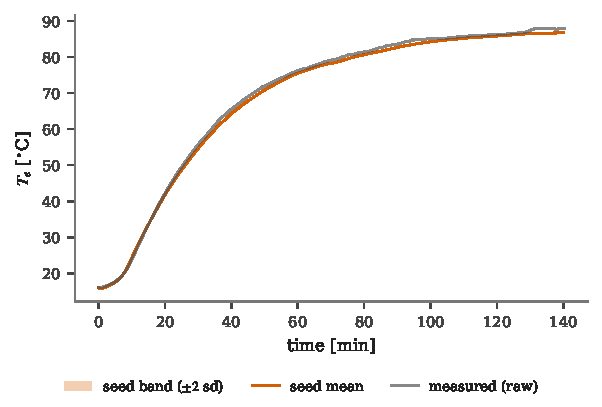
\includegraphics[width=0.6\textwidth]{fig9_bands.pdf}
\caption{Seed-ensemble band (10 PINN seeds, mean $\pm$ 2 sd) on the held-out Run 3 EOHP evaporator temperature:
the parameter band is far narrower than the residual -- seed spread quantifies identifiability, not total error.}
\label{fig:bands}
\end{figure}

The 10-seed ensemble spread of held-out rollouts is \SIrange{0.01}{0.05}{\kelvin} (2 sd), while actual held-out residuals
are \SIrange{0.25}{0.89}{\kelvin} (Fig.~\ref{fig:bands}): nominal 95\% bands cover 0--34\% of the raw data. Seed dispersion
quantifies parameter (identifiability) uncertainty only; the residual is dominated by structural and measurement
error. We therefore report seed bands as parameter uncertainty, not as full predictive bands (conformal augmentation
is future work).

\section{Discussion}
The consistent picture across Table~\ref{tab:loro} is that extrapolation is enabled by imposing a correct
(low-dimensional, linear) structure and fitting it by output-error shooting, not by physics-inspired optimisation
machinery and not by the physical parameterisation itself: the shooting fit of the same equations matches or beats
the PINN, a one-node variant does as well on the evaporator, and an unconstrained per-fluid linear state-space
with no physical content does slightly better still (0.28/0.30/\SI{0.68}{\kelvin}). The physical model's yield is
accordingly not accuracy but parsimony (9 shared parameters against $3{\times}8$ fitted independently per fluid)
and interpretability -- the dimensionless $R^*$, which the free form does not expose. This is a caution
for the PINN literature on small lumped systems -- where the classical shooting fit is trivially available -- and
a clarification of what grey-box structure buys in thermal identification. It is also a caution about black-box
surrogates for design: every generic learner, including a recurrent model trained on dynamics, failed the
extrapolation question that the structured model answers at sub-kelvin accuracy -- though a trivial constant-gap
predictor already achieves \SI{3}{\kelvin}, so the practical margin over naive baselines is modest and should be
stated. The scientific yield
is a dimensionless coupling ratio per fluid, robust to sampling, seed and method, that orders the fluids and tracks
the ethanol dry-out signature reported in the source data; the adiabatic channel offers a weak but free consistency
check on the identified states.

\textbf{Limitations.} One geometry; three fluids; effectively one independent driver per fold (the three fluids
share the vessel trace); structure-selection choices were made with all folds in view; slow heating ramps
(quasi-steady oscillation statistics are not resolved at \SI{5}{\second}); equal vessel--evaporator coupling
assumed across pipes, though the source reports fluid-dependent contact resistance, so the $R^*$ ordering cannot be
attributed to the pipe alone; the constant-parameter model cannot represent dry-out onset, which the source study
identifies as decisive for fluid choice; absolute fluxes are not identifiable from these records (the dataset's
derived flux constant $h=\SI{2100}{\watt\per\square\metre\per\kelvin}$ could not be traced to a source, and the
derived vessel-flux columns reproduce the cylindrical-wall conductance but are thermocouple-resolution-limited);
the known MOHP Run 3 flow-state change and hot-slug transient are left in (excluding $\pm$150\,s windows changes
that fold's RMSE only marginally). Results do not extend to hotspot-flux, dry-out-limited or geometry-optimisation
questions.

\section{Conclusion}
A two-node, vessel-driven grey-box model of a helically coiled OHP, identified by PINN or plain ODE shooting from a
public three-fluid dataset, predicts unseen runs at \SIrange{0.24}{0.85}{\kelvin}, including extrapolation
$\pm$\SI{23}{\kelvin} in heating level where all nonlinear black-box baselines fail; the identified right-hand side
exports as ONNX, remains consistent with an untrained adiabatic channel, and yields a dimensionless coupling ratio
$R^*$ that is robust across methods, seeds and sampling, and whose ethanol drift matches the dry-out signature
reported in the source data. The honest accounting: structure, not the optimiser, carries the accuracy; the second
node is justified by the auxiliary channels rather than evaporator accuracy; and the model's scenario implications
are illustrations within its validated envelope, not fluid recommendations.

\section*{Data availability}
All results derive from the public dataset of \cite{dataset} (Mendeley Data, DOI 10.17632/wnf5jwzp3c.3, CC BY 4.0).
Code, fitted parameters, ONNX models and result files are archived at [Zenodo DOI upon publication].

\begin{thebibliography}{99}\small
\bibitem{dataset} S.~K.~Yeboah, J.~Darkwa, Dataset on Helically Coiled Oscillating Heat Pipe (HCOHP),
Mendeley Data, v3, DOI 10.17632/wnf5jwzp3c.3 (CC BY 4.0).
\bibitem{dib} S.~K.~Yeboah, J.~Darkwa, Experimental data on Helically Coiled Oscillating Heat Pipe (HCOHP)
design and thermal performance, Data in Brief 33 (2020) 106505. doi:10.1016/j.dib.2020.106505.
\bibitem{ijts} S.~K.~Yeboah, J.~Darkwa, Theoretical and experimental investigation of a helically coiled
oscillating heat pipe, Int.\ J.\ Thermal Sciences 131 (2018) 531--544. doi:10.1016/j.ijthermalsci.2018.02.014.
\bibitem{ma2015} H.~B.~Ma, Oscillating Heat Pipes, Springer, New York, 2015. doi:10.1007/978-1-4939-2504-9.
\bibitem{li2019} Q.~Li, Y.~Wang, C.~Lian, H.~Li, X.~He, Effect of micro encapsulated phase change material on the
anti-dry-out ability of pulsating heat pipes, Applied Thermal Engineering 159 (2019) 113854.
doi:10.1016/j.applthermaleng.2019.113854.
\bibitem{ljung} L.~Ljung, System Identification: Theory for the User, 2nd ed., Prentice Hall, 1999.
\bibitem{gutenkunst} R.~N.~Gutenkunst, J.~J.~Waterfall, F.~P.~Casey, K.~S.~Brown, C.~R.~Myers, J.~P.~Sethna,
Universally sloppy parameter sensitivity in systems biology models, PLoS Computational Biology 3 (2007) e189.
\bibitem{raissi} M.~Raissi, P.~Perdikaris, G.~E.~Karniadakis, Physics-informed neural networks: a deep learning
framework for solving forward and inverse problems involving nonlinear partial differential equations,
J.\ Comput.\ Phys.\ 378 (2019) 686--707.
\bibitem{karniadakis} G.~E.~Karniadakis, I.~G.~Kevrekidis, L.~Lu, P.~Perdikaris, S.~Wang, L.~Yang,
Physics-informed machine learning, Nature Reviews Physics 3 (2021) 422--440.
\bibitem{wang2021} S.~Wang, Y.~Teng, P.~Perdikaris, Understanding and mitigating gradient flow pathologies in
physics-informed neural networks, SIAM J.\ Sci.\ Comput.\ 43 (2021) A3055--A3081.
\bibitem{brunton} S.~L.~Brunton, J.~L.~Proctor, J.~N.~Kutz, Discovering governing equations from data by sparse
identification of nonlinear dynamical systems, PNAS 113 (2016) 3932--3937.
\bibitem{gp} C.~E.~Rasmussen, C.~K.~I.~Williams, Gaussian Processes for Machine Learning, MIT Press, 2006.
\bibitem{vovk} V.~Vovk, A.~Gammerman, G.~Shafer, Algorithmic Learning in a Random World, Springer, 2005.
\end{thebibliography}

\end{document}
